\chapter{Projekt}
Rozdział ten zawiera szkice rozwiązań dla wymagań z~poprzednich rozdziałów.

\section{Uniwersalny silnik}
\subsection{Podział na warstwy}
Zdecydowałem się podzielić wykres na pięć warstw. Odrysowywanie wykresu będzie się składało z~odrysowania zawartości każdej z~warstw, począwsze od tła, a~na pierwszym planie skończywszy.
Układ warstw został przedstawiony na rysunku~\ref{rys:warstwy}.

\begin{figure}
\centering
\caption{Warstwy wykresu}\label{rys:warstwy}
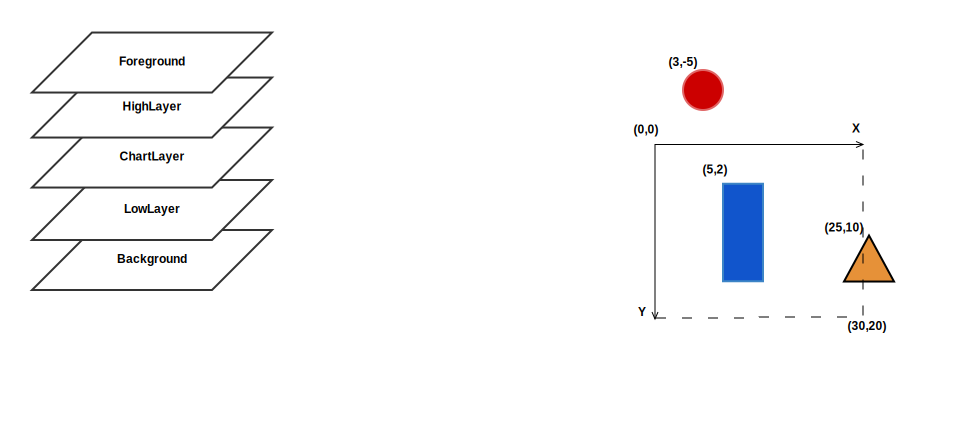
\includegraphics{img/warstwy.png}
\end{figure}

Warstwy tła oraz pierwszego planu służą jedynie odrysowywaniu wzorów przekazanych za pomocą pędzla. Pozostałe warstwy są bardziej złożone i~zawierają liczne elementy.

Warstwy niska i~wysoka są odrysowywane zgodnie z~algorytmem malarza. Służą dodawaniu przez programistów własnych elementów do wykresów istniejących klas.

Warstwa wykresu służy odrysowaniu głównej zawartości wykresu. Tym etapem steruje strategia danego wykresu. W~ogólnym przypadku programiści nie powinni dodawać własnych elementów do tej warstwy.

\subsubsection{Wskazówki implementacyjne}
Metoda odpowiedzialna za odrysowywanie wykresu powinna być \textit{Metodą Szablonową}~\cite[264-268]{Patterns}, czyli niewirtualną, publiczną metodą klasy bazowej, wywołującą kolejne metody odpowiedzialne za odrysowanie pojedynczych warstw. Metody te powinny z~kolei być wirtualne i~chronione.
Metody odpowiedzialne za tło i~pierwszy plan powinny udostępniać domyślną implementację, natomiast pozostałe powinny być czysto wirtualne.

\subsection{Lokalny system współrzędnych}
Wykresy będą posiadać lokalny, kartezjański układ współrzędnych rzeczywistych. Ułatwi to realizację takich wymagań jak: skalowanie wykresu czy interaktywność. 

\begin{figure}
\centering
\caption{Lokalny układ współrzędnych}\label{rys:uklad:wspolrzednych}
\includegraphics{img/uklad_wspolrzednych.png}
\end{figure}

Ponadto każdy wykres będzie posiadał prostokąt określający jego zakres. Pozwoli to na optymalizację polegającą na pominięciu renderowania elementów spoza tego prostokąta.

\subsection{Diagramy klas}
Ogólna koncepcja na strukturę wykresu została przedstawiona na diagramie~\ref{rys:klasy:top_level}.

Klasy pochodne od QocAbstractChart są miejscem łączącym wszystkie inne elementy. To na nich będą ustawiane parametry odnoszące się do całości wykresu, np. włączenie antyaliasingu.

QocSeries odpowiada za dane dostarczane do wykresu. Jest lekkim odpowiednikiem modelu z~architektury Model-Widok.

QocAbstractStrategy to klasa bazowa dla strategii -- layoutu, odpowiedzialnego za odpowiednie układanie elementów wykresu, głównie z~warstwy środkowej -- \textit{ChartLayer}, i~ich odrysowywanie. Jest to szczególnie przydatny komponent dla wykresów, które mogą być budowane na różne sposoby, np. wykres słupkowy.


\begin{figure}
\centering
\caption{Diagram top level}\label{rys:klasy:top_level}
\includegraphics[scale=0.5]{img/klasy-top_level.png}
\end{figure}


\section{Qt Quick}

\subsection{Eksport klas C++ do QML}
Klasy wszystkich wysokopoziomowych elementów powinny być pochodnymi klasy QObject. Wszelkie ich parametry, które powinny być konfigurowane przez programistów należy włączyć do zbioru właściwości tej klasy. W~szczególności należy zadbać o~to, aby przy zmianie wartości danej właściwości, i~tylko wtedy, emitować sygnał informujący o~tym zdarzeniu. Jest to niezbędne do poprawnego działania mechanizmu wiązania w~QML. Ponadto, wszystkie metody, które powinny być dostępne z~QML, a~nie są slotami, powinny zostać opatrzone makrem \textit{Q\_INVOKABLE}.

Większość klas powinna być gotowa do wyeksportowania ich do QML za pomocą standardowej procedury, np. poprzez wywołanie funkcji szablonowej
\begin{lstlisting}
template<typename T>
int qmlRegisterType(const char *uri, int versionMajor, 
		    int versionMinor, const char *qmlName)
\end{lstlisting}
Parametrem szablonu jest eksportowany typ, a~parametry funkcji to nazwa modułu, dwie liczby odpowiadające za wersję modułu oraz nazwa pod jaką będzie dostępna eksportowana klasa z~poziomu QML. Qt udostępnia jeszcze kilka innych, specjalizowanych szablonów, np. dla singletonów.\newline

Pozostałe klasy, do wykorzystania ich w~QML, będą wymagały specjalnych interfejsów. Dla klas związanych z~GUI, bazujących na QPainter będzie to QQuickPaintedItem, a~dla tych wykorzystujących SceneGraph -- QQuickItem.

\subsection{Uproszczone interfejsy}
Zakładam, że w~niektórych przypadkach interfejsy dostępne z~poziomu QML mogą, a~nawet powinny być uboższe od swoich odpowiedników w~C++. Najlepszym przykładem będzie ramka wokół dowolnego elementu graficznego, będącego składową wykresu. Z~poziomu C++ powinna istnieć możliwość ustawienia pióra używanego do jej odrysowania. Klasa pióra, czyli \textit{QPen}, nie dziedziczy po \textit{QObject}, więc nie może być dostępna w~QML.

Jednym z~rozwiązań tego problemu jest stworzenie specjalnych adapterów dla wszystkich klas nie spokrewnionych z~\textit{QObject}, które wykrzystam w~swojej bibliotece. Wolę jednak przyjąć konwencję stosowaną w~Qt~Quick i~ograniczyć, uprościć interfejsy moich klas dla QML, tak aby możliwe było tam zmienianie tylko najważniejszych parametrów. W~przypadku ramki będą to grubość oraz kolor. Jednocześnie z~poziomu C++ cały czas będzie można zmienić wszystkie parametry pióra odrysowujacego daną ramkę.

\section{Interaktywność}
Klasy wykresów muszą udostępniać metody mapujące globalne współrzędne na wartości lokalne i~odwrotnie. Ponadto każdy z~elementów wykresu musi posiadać metody:
\begin{itemize}
\item{boundingRect(), zwracająca najmniejszy prostokąt opisujący dany element.}
\item{shape(), zwracająca kształt elementu zapisany jako \textit{QPainterPath}.}
\end{itemize}

\section{Skalowanie}
Każdy z~widoków, do których zostanie podpięty wykres, ma obowiązek powiadomienia wykresu o zmianie swojego położenia lub rozmiaru. Jest to niezbędne w~celu poprawnej implementacji automatycznego skalowania wykresu oraz mapowania współrzędnych globalne -- lokalne.

\subsubsection{Wskazówki implementacyjne}
Klasa bazowa wykresów powinna posiadać właściwość typu prostokąt, opisującą geometrię widoku podłączonego do danego wykresu. Zmiana tej właściwości powinna się odbywać poprzez odpowiedni slot, przyjmujący jako argument nowy prostokąt.

W~zależności od klasy, z~której wywodzi się widok podłączony do wykresu, slot powiadamiający wykres o~zmianie geometrii widoku powinien być wywoływany następujących metodach widoku:
\begin{itemize}
\item{QWidget}
	\begin{itemize}
	\item{moveEvent()}
	\item{resizeEvent()}
	\end{itemize}
\item{QGraphicsItem}
	\begin{itemize}
	\item{prepareGeometryChange()}
	\end{itemize}
\item{QTextFrame}

\item{QQuickItem}
	\begin{itemize}
	\item{geometryChanged()}
	\end{itemize}
\end{itemize}

\section{Zależności między plikami}
Mogłoby się wydawać, że każde nowe wydanie Qt powinno wymagać ponownej kompilacji projektów zeń korzystających. Tak jednak nie jest. Twórcy Qt zadbali o~to, aby zawsze wtedy, kiedy to możliwe, zachowana była zgodność binarna. Oznacza to, że jeśli przy poprawkach do nowej wersji nie zostały zmienione nagłówki klas, a~jedynie ich implementacje, to przebudowanie całej aplikacji nie jest konieczne. Teoretycznie przejście z~Qt~w~wersji 4.8.3 na wersję 4.8.4 może odbyć się jedynie poprzez podmianę plików .dll. Temat zgodności binarnej oraz zależności czasu kompilacji międzi plikami został poruszony przez Scotta Meyersa~\cite[150-158]{50Ways}.

\subsection{QObject}
Klasa QObject została zaprojektowana jako \textit{Most}~\cite[181-190]{Patterns}, zmodyfikowany o~posiadany przez ciało wskaźnik do uchwytu. Podział na uchwyt i~ciało zmniejsza zależności pomiędzy plikami bibliotek Qt i~znacząco skraca czas kompilacji po zmianach w~kodzie. Dodatkowo QObject posiada konstruktor przyjmujący jako argument wskaźnik do ciała, dzięki czemu można je zaalokować tylko raz, w~klasie najniższego poziomu hierarchii dziedziczenia, a~następnie przekazać jako argument konstruktora klasy bazowej. 
Koncepcję \textit{Mostu} zobrazowałem w~kontekście mojej biblioteki na rys.~\ref{rys:dpointer}.\newline

\begin{figure}
\centering
\caption{Przykładowa hierarchia klas}\label{rys:dpointer}
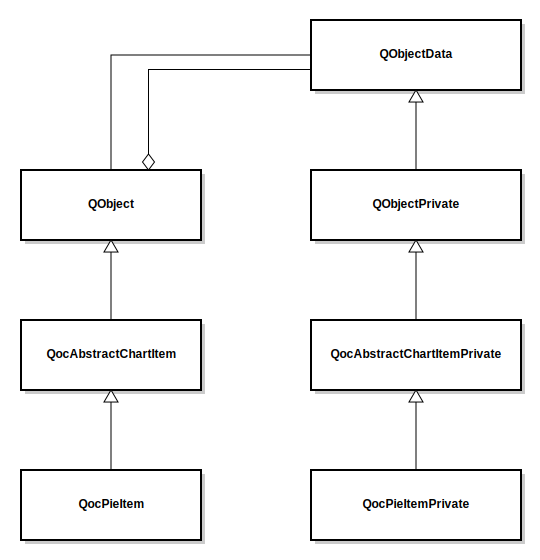
\includegraphics[scale=0.8]{img/dpointer.png}
\end{figure}

W~Qt przyjęto następującą koncepcję nazewniczą:
\begin{itemize}
\item{uchwyt ma standardową nazwę, zgodną ze swoim przeznaczeniem,}
\item{ciało ma nazwę składającą się z~nazwy odpowiadającego mu uchwytu oraz sufiksu ,,Private''.}
\end{itemize}


\subsection{Dostęp do uchwytów i ciał}
Podejście opisane w~poprzednim punkcie skutkuje jednak powstaniem pewnego efektu ubocznego.
Wskaźniki do uchwytu i~ciała są typów klas znajdujących się na szczycie hierarchii dziedziczenia. Dostęp do metod klas pochodnych niewystępujących w~klasach bazowych wymaga rzutowania w~dół. 
Problem ten rozwiązano za pomocą czterech makrodefinicji przyjmujących jako argument nazwę klasy uchwytu. Dwie z~nich należy wywołać w~odpowiednich nagłówkach. Z~kolei pozostałe dwie należy wywoływać na początku każdej metody wymagającej odwołania do ciała lub uchwytu. Miejsce wykorzystania konkretnych makr podaję w~tabelce~\ref{tab:makra}. Technika ta została szczegółowo opisana w~artykule~\footnote{QObject -- Most \url{http://qt-project.org/wiki/Dpointer}}

\begin{table}[h]\footnotesize
\centering
\caption{Makrodefinicje}
\label{tab:makra}
\begin{tabular}{|c|c|c|}
\hline
Miejsce & Uchwyt & Ciało\\
\hline
Nagłówek & Q\_DECLARE\_PRIVATE & Q\_DECLARE\_PUBLIC\\
\hline
Metoda & Q\_D & Q\_Q\\
\hline
\end{tabular}
\end{table}
